\documentclass[10pt,final,leqno]{beamer}

%\usetheme{CambridgeUS}
\usetheme[style=ntnu,language=en]{ntnu2015}
%\usecolortheme{orchid}

\usepackage[utf8]{inputenc}
\usepackage[T1]{fontenc}

% Paths
\newcommand{\figs}{../figs}
\newcommand{\data}{../data}
\newcommand{\code}{../code}

% URL styles
\usepackage{url}
\urlstyle{sf}

% Units
\usepackage[detect-weight=true, binary-units=true]{siunitx}
\DeclareSIUnit\flop{FLOPS}

% Math
\usepackage{amsmath}
\usepackage{amssymb}
\usepackage{bm}
\usepackage{nicefrac}
\newcommand{\dif}[1]{{\;\text{d}#1}}

% Graphics
\usepackage{graphicx}
\usepackage{caption}
%\usepackage{subcaption}
\graphicspath{{../figs/}}

% Tikz
\usepackage{tikz}
\usetikzlibrary{positioning,shapes,arrows,calc,intersections}
\usepackage{pgfplots}
\usepgfplotslibrary{dateplot}
\pgfplotsset{compat=1.14} 

% Colors
\definecolor{darkblue}{HTML}{00688B}
\definecolor{darkgreen}{HTML}{6E8B3D}
\definecolor{cadet}{HTML}{DAE1FF}
\definecolor{salmon}{HTML}{FFB08A}

\usepackage{algorithm}

% Listings
\usepackage{textcomp}
\usepackage{listings}
\lstset{
  keywordstyle=\bfseries\color{orange},
  stringstyle=\color{darkblue!80},
  commentstyle=\color{darkblue!80},
  showstringspaces=false,
  basicstyle=\ttfamily,
  upquote=true,
}
\lstdefinestyle{fortran}{
  language=Fortran,
  morekeywords={for},
  deletekeywords={status},
}
\lstdefinestyle{c}{
  language=C,
  morekeywords={include},
}
\lstdefinestyle{glsl}{
  language=C,
  morekeywords={attribute, vec2, vec3, vec4, varying, uniform, mat2, mat3, mat4},
}
\lstdefinestyle{cuda}{
  language=C,
  morekeywords={__global__, __device__, __host__, __shared__},
}
\lstdefinestyle{shell}{
  language=bash,
  morekeywords={mkdir, ssh, cmake},
}

% Double hlines
\usepackage{hhline}

% Misc
\usepackage{nth}

\subtitle{TMA4280---Introduction to Supercomputing}

\graphicspath {{../figs/}}

\AtBeginSection[]
{
 \begin{frame}<beamer>
 \frametitle{Outline}
 \tableofcontents[currentsection]
 \end{frame}
}

\begin{document}


\title{The Message Passing Interface (MPI)}
\institute{NTNU, IMF}
\date{February 02. 2018}
%\author{Aurélien Larcher}

\maketitle

\begin{frame}
  \frametitle{Recap: Multiprocessors}

Shared Memory Multi-Processors(SMMPs)
  \begin{center}
    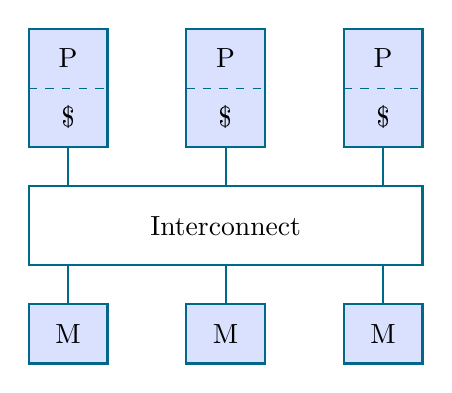
\begin{tikzpicture}[scale=0.5]
  \foreach \i in {0,4,8}
  {
    \draw[darkblue, fill=cadet, thick] (\i,10) rectangle (\i+2,7);
    \draw[darkblue, very thin, dashed] (\i,8.5) -- (\i+2,8.5);
    \draw[darkblue, fill=cadet, thick] (\i,3) rectangle (\i+2,1.5);
    \draw[darkblue, thick] (\i+1,7) -- (\i+1,6);
    \draw[darkblue, thick] (\i+1,3) -- (\i+1,4);
    \node at (\i+1,9.25) {P};
    \node at (\i+1,7.75) {\$};
    \node at (\i+1,2.25) {M};
  }
  \draw[darkblue, thick] (0,6) rectangle (10,4);
  \node at (5,5) {Interconnect};
\end{tikzpicture}

  \end{center}

Any processor can take a memory reference anywhere (with or without a latency difference due to locality).
\end{frame}

\begin{frame}
  \frametitle{Recap: Multiprocessors}
Shared Memory architecture:
\begin{itemize}
\item physical address space for all processors:  global shared address space 
\item different solutions: SMP/UMA, DSM/NUMA
\item cache coherency issue
\item access to shared data needs protection (resource locking)
\end{itemize}

\medskip
\textcolor{red}{Pitfalls}: 
\begin{itemize}
\item lack of scalability CPU vs Memory (memory contention)
\item complexity of design safe and efficient memory access
\end{itemize}
\end{frame}

\begin{frame}
  \frametitle{Recap: Multiprocessors}

Distributed Memory Multi-Processors (DMMPs)
  \begin{center}
    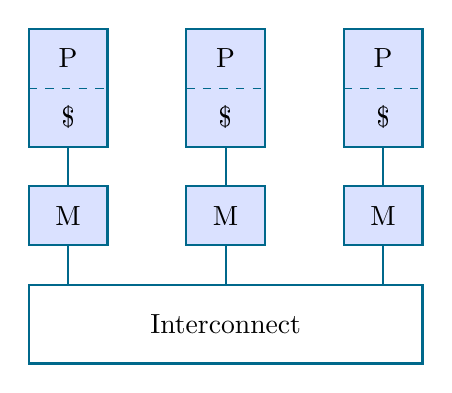
\begin{tikzpicture}[scale=0.5]
  \foreach \i in {0,4,8}
  {
    \draw[darkblue, fill=cadet, thick] (\i,10) rectangle (\i+2,7);
    \draw[darkblue, very thin, dashed] (\i,8.5) -- (\i+2,8.5);
    \draw[darkblue, fill=cadet, thick] (\i,6) rectangle (\i+2,4.5);
    \draw[darkblue, thick] (\i+1,7) -- (\i+1,6);
    \draw[darkblue, thick] (\i+1,3.5) -- (\i+1,4.5);
    \node at (\i+1,9.25) {P};
    \node at (\i+1,7.75) {\$};
    \node at (\i+1,5.25) {M};
  }
  \draw[darkblue, thick] (0,1.5) rectangle (10,3.5);
  \node at (5,2.5) {Interconnect};
\end{tikzpicture}

  \end{center}
Processor cannot take memory reference to the entire memory space: communication through an interconnect is required for "remote" memory.
\end{frame}

\begin{frame}
  \frametitle{Recap: Multiprocessors}
Distributed Memory architecture:
\begin{itemize}
\item each processor has a private physical address space
\item hardware send/receive messages to communicate between processors
\item scalability of memory (add nodes)
\end{itemize}

\medskip
\textcolor{red}{Pitfalls}:
\begin{itemize}
\item need to implement data exchange between processors
\item memory latency difference between local memory and remote memory
\item fault tolerance
\end{itemize}
\end{frame}

\begin{frame}
  \frametitle{Parallelism}

How to solve a problem in parallel?

\medskip
\begin{itemize}

\item Decomposition of the data provided or domain onto which the problem is posed:
\textcolor{blue}{Data Parallelism}

\medskip
Example: Mesh partitioning (data distribution techniques)

\medskip
$\rightarrow$ scales with the data (more potential compared to task parallelism)

\vspace{2ex}
\item Decompose the execution into several tasks according to the work to be done: \textcolor{blue}{Function/Task Parallelism}

\medskip
Example: Multiple models


\medskip
$\rightarrow$ scales only with the number of logical functions/tasks

\end{itemize}

\medskip
Both models can be combined, and will be limited respectively by models and data dependencies.

\end{frame}

\begin{frame}
  \frametitle{Implementation}

\textcolor{blue}{Single Program Multiple Data} (SPMD)
\begin{itemize}
\item single program executed by all processors simultaneously
\item the same or different instructions can be executed
\item several data streams can come into play
\end{itemize}
This is the most common case. 

\medskip
A program is executed in parallel on each processor:
\begin{center}
    \scalebox{0.8}{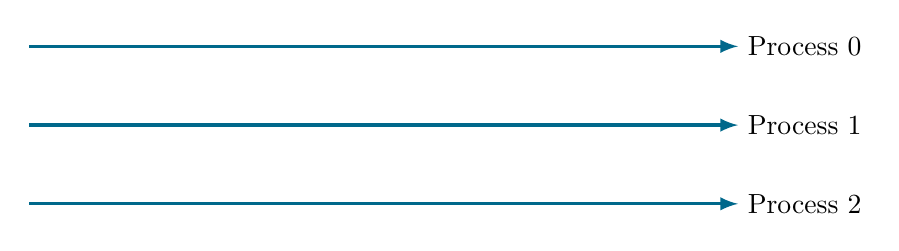
\begin{tikzpicture}
  \foreach \i in {0,...,2} {
    \draw[darkblue, very thick, -latex] (0,-\i) -- (9,-\i);
    \node[anchor=west] at (9,-\i) {Process \i};
  }
\end{tikzpicture}
}
\end{center}

\bigskip
\textcolor{blue}{Multiple Programs Multiple Data} (MPMD)

\medskip
$\rightarrow$ multiple programs can be combined to solve a problem.

\end{frame}

\begin{frame}
  \frametitle{Programming Model for Distributed Memory}
Requirement: Programming model to take advantage of distributed memory architectures:


\begin{center}
\textcolor{red}{Distinguish Computer Architecture and Programming Model}:\\
``a programming model is a view of the memory model''
\end{center}

\medskip
Concept of Message Passing: definition of an object model to represent the execution of the program

\medskip
\begin{itemize}
\item Encapsulation: the layer provides general facilities that can be used without knowledge of the implementation.
\item Distribution:
\begin{enumerate}
\item synchronous: sender/receiver wait until data has been sent/received
\item asynchronous: sender/receiver can proceed after sending/receiving is intiated 
\end{enumerate}
\end{itemize}
\medskip

\end{frame}

\begin{frame}
  \frametitle{The message passing model}
  \begin{center}
    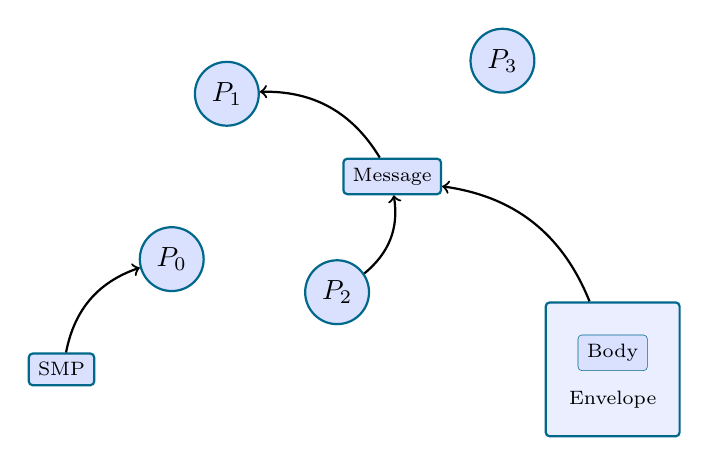
\begin{tikzpicture}[
  proc/.style={shape=circle, draw=darkblue, fill=cadet, thick},
  msg/.style={shape=rectangle, draw=darkblue, fill=cadet, thick, rounded corners=0.5mm},
  env/.style={minimum height=1.7cm, minimum width=1.7cm},
  scale=0.7,
  ]
  \node[proc] (p0) at (0,0) {$P_0$};
  \node[proc] (p1) at (1,3) {$P_1$};
  \node[proc] (p2) at (3,-0.6) {$P_2$};
  \node[proc] (p3) at (6,3.6) {$P_3$};
  \node[msg] (msg) at (4.0, 1.5) {\scriptsize Message};
  \node[msg, env, fill=cadet!55] (env) at (8, -2.0) {};
  \node[msg, very thin] (body) at (8, -1.7) {\scriptsize Body};
  \node[below of=body, node distance=6mm] {\scriptsize Envelope};
  \draw[->, thick] (p2) edge[bend right] node [right] {} (msg);
  \draw[->, thick] (msg) edge[bend right] node [right] {} (p1);
  \draw[->, thick] (env) edge[bend right] node [right] {} (msg);

  \node[msg] (smp) at (-2,-2) {\scriptsize SMP};
  \draw[->, thick] (smp) edge[bend left] node [right] {} (p0);
\end{tikzpicture}

  \end{center}

\begin{itemize}
\item SMMPs do not \textbf{need} a message passing model but \textbf{can} use it.
\item DMMPs \textbf{require} a message passing model.
\end{itemize}
\end{frame}

\begin{frame}
  \frametitle{DMMP: nodes interconnected by a network}
  Examples: 2D mesh or toroid. Vilje is an eight-dimensional hyper-cube (!).
  \begin{center}
    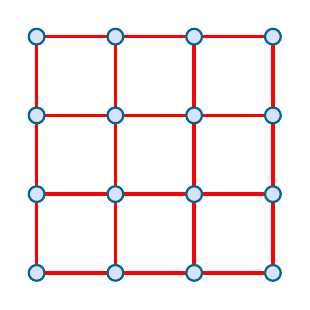
\begin{tikzpicture}
  \foreach \i in {0,...,3} {
    \draw[very thick, red] (\i,0) -- (\i,3);
    \draw[very thick, red] (0,\i) -- (3,\i);
  }
  \foreach \i in {0,...,3} {
    \foreach \j in {0,...,3} {
      \draw[thick, darkblue, fill=cadet] (\i,\j) circle (0.1);
    }
  }
\end{tikzpicture}

    \qquad
    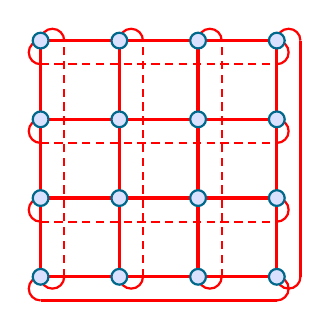
\begin{tikzpicture}
  \foreach \i in {0,...,3} {
    \draw[very thick, red] (\i,0) -- (\i,3);
    \draw[very thick, red] (0,\i) -- (3,\i);
  }
  \foreach \i in {0,...,3} {
    \draw[thick, red] (\i,0) arc (180:360:0.15);
    \draw[thick, red] (\i+0.3,3) arc (0:180:0.15);
    \draw[thick, red] (0,\i) arc (90:270:0.15);
    \draw[thick, red] (3,\i-0.3) arc (270:450:0.15);
  }
  \foreach \i in {0,...,2} {
    \draw[thick, red, densely dashed] (\i+0.3,0) -- (\i+0.3,3);
    \draw[thick, red, densely dashed] (0,\i+0.7) -- (3,\i+0.7);
  }
  \draw[thick, red] (3.3,0) -- (3.3,3);
  \draw[thick, red] (0,-0.3) -- (3,-0.3);
  \foreach \i in {0,...,3} {
    \foreach \j in {0,...,3} {
      \draw[thick, darkblue, fill=cadet] (\i,\j) circle (0.1);
    }
  }
\end{tikzpicture}

  \end{center}

A subset of the given DMMP used for solving a problem, consists of:
\begin{itemize}
\item a group of processors (SMMPs) identified uniquely,
\item executing tasks simultaneaously,
\item and communicating data by passing messages.
\end{itemize}

\medskip
$\rightarrow$ Performance factors: data dependencies, amount of data, communication pattern, network topology, \dots

\end{frame}


\begin{frame}
  \frametitle{The message passing model}

Data communication may or may not involve all the processors with each other:
\begin{enumerate}
\item one-to-one
\item one-to-all
\item all-to-one
\item all-to-all
\end{enumerate}

\bigskip
Intuitively, the message body will express different properties of the data:
\begin{enumerate}
\item Location,
\item Nature,
\item Amount.
\end{enumerate}

\medskip
The recipient of the message, a tag (to identify the message), and other possible metadata to determine how the data will be exchanged.

\end{frame}

\begin{frame}
\frametitle{Basic idea of Message Passing: Point-to-Point}

\begin{center}
\texttt{send(address, length, destination, tag)}
\end{center}

\begin{tabular}{|c|l|}
\hline
\texttt{address}    & memory location defining the begining of the buffer\\
\texttt{length}     & length in bytes of the send buffer\\
\texttt{destination}& receiving process rank\\
\texttt{tag}        & arbitrary identifier \\
\hline
\end{tabular}

\begin{center}
\texttt{recv(address, maxlength, source, tag, status)}
\end{center}

\begin{tabular}{|c|l|}
\hline
\texttt{address}    & memory location defining the begining of the buffer\\
\texttt{maxlength}  & maxlength in bytes of received data\\
\texttt{destination}& sending process rank\\
\texttt{tag}        & arbitrary identifier \\
\texttt{status}     & metadata: actual length \\
\hline
\end{tabular}

\end{frame}

\begin{frame}
  \frametitle{MPI: Message Passing Interface}
Distributed memory architecture do not offer a shared address space
\begin{itemize}
\item a processor cannot get a memory reference from any location in the system
\item a software layer is required to provide an abstraction for exchanging data between processors
\end{itemize}

\medskip
The Message Passing Interface (MPI) specifies how a library should provide such facilities.

\medskip
MPI is a \textbf{specification}, several implementations available:
\begin{itemize}
\item MPICH (Argonne National Laboratory)
\item OpenMPI
\item Vendor specific: Cray, Intel, etc \dots
\end{itemize}
\end{frame}

\begin{frame}
  \frametitle{MPI: Message Passing Interface}
  Advantages of the MPI message-passing model:
  \begin{itemize}
  \item standardization,
  \item portability,
  \item performance,
  \item expressiveness.
  \end{itemize}

  MPI 1.0 is a specification comprising about 128 functions or operations:
  \begin{itemize}
  \item \textcolor{red}{one-to-one} operations (or point-to-point communication);
  \item \textcolor{red}{one-to-all} operations;
  \item \textcolor{red}{all-to-one} operations;
  \item \textcolor{red}{all-to-all} operations.
  \end{itemize}
  The last three types are referred to as {\em collective} operations.
\end{frame}

\begin{frame}[fragile]
  \frametitle{Header file}

\begin{center}
Interface described in the header file.
\end{center}

For C:
\begin{lstlisting}[style=c]
#include "mpi.h"
\end{lstlisting}

  And for Fortran:
\begin{lstlisting}[style=fortran]
include 'mpif.h'
\end{lstlisting}
\end{frame}

\begin{frame}[fragile]
  \frametitle{Calling functions}
  For C:
\begin{lstlisting}[style=c,morekeywords={err}]
err = MPI_Xxxxx(parameters, ...);
\end{lstlisting}
  Or ignoring the error code:
\begin{lstlisting}[style=c,morekeywords={err}]
MPI_Xxxxx(parameters, ...);
\end{lstlisting}

  For Fortran, everything is a subroutine:
\begin{lstlisting}[style=fortran,morekeywords={err}]
call MPI_XXXXX(parameters, ..., err)
\end{lstlisting}

\medskip
MPI objects are internal and accessed via handles to ensure transparency: do not expose implementation details.
\end{frame}

\begin{frame}
  \frametitle{MPI: Six essential functions}
  \begin{center}
    \bgroup\def\arraystretch{1.2}
    \addtolength{\tabcolsep}{0.5cm}
    \begin{tabular}{ll}
      \hline
      C & Fortran  \\
      \hhline{==}
      \texttt{MPI\_Init} & \texttt{call MPI\_Init} \\
      \texttt{MPI\_Comm\_size} & \texttt{call MPI\_Comm\_size} \\
      \texttt{MPI\_Comm\_rank} & \texttt{call MPI\_Comm\_rank} \\
      \texttt{MPI\_Send} & \texttt{call MPI\_Send} \\
      \texttt{MPI\_Recv} & \texttt{call MPI\_Recv} \\
      \texttt{MPI\_Finalize} & \texttt{call MPI\_Finalize} \\
      \hline
    \end{tabular}
    \addtolength{\tabcolsep}{-0.5cm}
    \egroup
  \end{center}

\medskip
$\rightarrow$ Look at the \texttt{mpi.h} header for example (usually in \texttt{/usr/include/mpi/})
\end{frame}

\begin{frame}
  \frametitle{MPI: Execution context}

The program is run in parallel using the \texttt{mpirun} (or \texttt{mpiexec}) utility: options can be passed to MPI using flags.

\medskip
A number of MPI \textbf{process} is created: each of them executes an instance of the program.

\medskip
On each process MPI should be initialized at the beginning, and finalize at the end of the execution (once!):
\begin{itemize}
\item \texttt{MPI\_Init}
\item  \texttt{MPI\_Finalize}
\end{itemize}

\medskip
All the MPI processes are part of a \textbf{group} \texttt{MPI\_Group} and can communicate via a \textbf{communicator} \texttt{MPI\_Comm}.

\medskip
The communication involves a number of processes, identified by a rank:
\begin{itemize}
\item \texttt{MPI\_Comm\_size}
\item \texttt{MPI\_Comm\_rank}
\end{itemize}
\end{frame}

\begin{frame}[fragile]
  \frametitle{Sample output with four processors}
  \begin{center}
    \begin{tabular}{c}
\begin{lstlisting}
Process 0: Hello, world!
Process 1: Hello, world!
Process 3: Hello, world!
Process 2: Hello, world!
\end{lstlisting}
    \end{tabular}
  \end{center}
  Note that output ordering is not guaranteed.

\medskip
\begin{center}
\textcolor{red}{But:} MPI is non-overtaking, message processed in order.
\end{center}
\end{frame}

\begin{frame}
  \frametitle{MPI: Message = data + envelope}

Implementation of Point-to-Point communication:

\medskip
  \texttt{\textcolor{red}{MPI\_Send}($\underbrace{buffer, count, datatype}_{\textcolor{blue}{data}}$,
    $\underbrace{dest, tag, comm}_{\textcolor{blue}{envelope}}$); } \\
  \texttt{\textcolor{red}{MPI\_Recv}($\underbrace{buffer, count, datatype}_{\textcolor{blue}{data}}$,
    $\underbrace{source, tag, comm,\&status}_{\textcolor{blue}{envelope}}$); }

  Examples of predefined data types (C):
  \begin{itemize}
  \item \texttt{MPI\_CHAR}
  \item \texttt{MPI\_INT}
  \item \texttt{MPI\_FLOAT}
  \item \texttt{MPI\_DOUBLE}
  \end{itemize}
\end{frame}

\begin{frame}[fragile]
  \frametitle{Message buffers}

\begin{center}
A \textit{buffer} is an array of \textbf{contiguous} values of a given data type,
\end{center}

\begin{itemize}
\item MPI defines several Basic Types,
\item data structures may not be contiguous in memory so copy is required,
\item MPI allows creation of \textit{ad hoc} data types using MPI Derived Types:

\begin{lstlisting}[style=c,morekeywords={MPI_Type_contiguous,MPI_Type_vector,MPI_Datatype}]
int MPI_Type_contiguous (
int count, // replication count
MPI_Datatype oldtype, // old datatype
MPI_Datatype * newtype ) // new datatype

int MPI_Type_vector (
int count , // number of blocks
int blocklength ,// number of elements per block
int stride , // number of elements between block
MPI_Datatype oldtype , // old datatype
MPI_Datatype * newtype ) // new datatype

\end{lstlisting}
\end{itemize}
\end{frame}


\begin{frame}[fragile]
\frametitle{Interprocess communication}

Execution of task is performed by MPI \textbf{MPI Processes}:
\begin{itemize}
\item MPI Processes belong to \textbf{Groups},
\item Each process is identified with a group by its \textbf{Rank},
\item MPI defines an object \textbf{Communicator} used by collection of processes to communicate.
\end{itemize}

\medskip
\begin{itemize}
\item \texttt{MPI\_COMM\_WORLD} is the main communicator \textit{i.e} it allows communication with all processes run with \texttt{mpirun},
\item a group+communicator consisting of a subset of \textit{all} processes may be created to:
\begin{itemize}
\item simplify the implementation,
\item assign specific tasks,
\item apply operators to a subset.
\end{itemize}
For example for Monte-Carlo simulations, $N$ perturbed problems may be solved in parallel.
\end{itemize}

\medskip
Synchronization can be done explicitely with a \textbf{Barrier} or implicitely using blocking routines.
\end{frame}


\begin{frame}[fragile]
  \frametitle{MPI with C}
  \scalebox{0.5}{
    \lstinputlisting[style=c]{\code/mpi_hello/c/hello.c}
  }
\end{frame}

\begin{frame}[fragile]
  \frametitle{MPI with Fortran}
  \scalebox{0.5}{
    \lstinputlisting[style=fortran]{\code/mpi_hello/fortran/hello.f90}
  }
\end{frame}

\begin{frame}[fragile]
  \frametitle{Point-to-point communication}
  \texttt{MPI\_Send} and \texttt{MPI\_Recv} are \emph{blocking}. Deadlock
  example:
  \begin{center}
    \begin{tabular}{c}
\begin{lstlisting}[style=c,morekeywords={MPI_Recv,MPI_Send}]
if (rank == 0) {
  MPI_Recv(...);
  MPI_Send(...);
}
else if (rank == 1) {
  MPI_Recv(...);
  MPI_Send(...);
}
\end{lstlisting}
    \end{tabular}
  \end{center}

\textbf{Deadlock}: execution hang due to incorrect scheduling of messages.

\end{frame}

\begin{frame}[fragile]
  \frametitle{Point-to-point communication}
  How to avoid deadlock?
  \begin{center}
    \begin{tabular}{c}
\begin{lstlisting}[style=c,morekeywords={MPI_Recv,MPI_Send}]
if (rank == 0) {
  MPI_Send(...);
  MPI_Recv(...);
}
else if (rank == 1) {
  MPI_Recv(...);
  MPI_Send(...);
}
\end{lstlisting}
    \end{tabular}
  \end{center}

\medskip
Pairwise \texttt{MPI\_Sendrecv} is usually preferred and may be optimized by vendors.

\end{frame}

\begin{frame}[fragile]
\frametitle{Communication modes}

MPI may provide several versions of a routine: different communication modes
\begin{itemize}
\item Synchronous: send blocks until handshake is done and matching receive has started.
\item Ready: send blocks until matching receive has started (no handshake).
\item Buffered: send returns as soon as data is buffered internally.
\item Standard: Synchronous or Buffered depending on message size and resources.
\end{itemize}

\medskip
Assuming synchronous mode is the safest to avoid hiding deadlocks.

\end{frame}

\begin{frame}[fragile]
  \frametitle{Collective operations}
  In general,
  \begin{itemize}
  \item Involves all of the processes in a group, and
  \item are more efficient and less tedious to use compared to point-to-point
    communication.
  \end{itemize}
  An example (synchronization between processes):
  \begin{center}
    \begin{tabular}{c}
\begin{lstlisting}[style=c,morekeywords={MPI_Barrier}]
MPI_Barrier(comm);
\end{lstlisting}
    \end{tabular}
  \end{center}
\end{frame}

\begin{frame}
  \frametitle{Collective operations}
  \begin{center}
    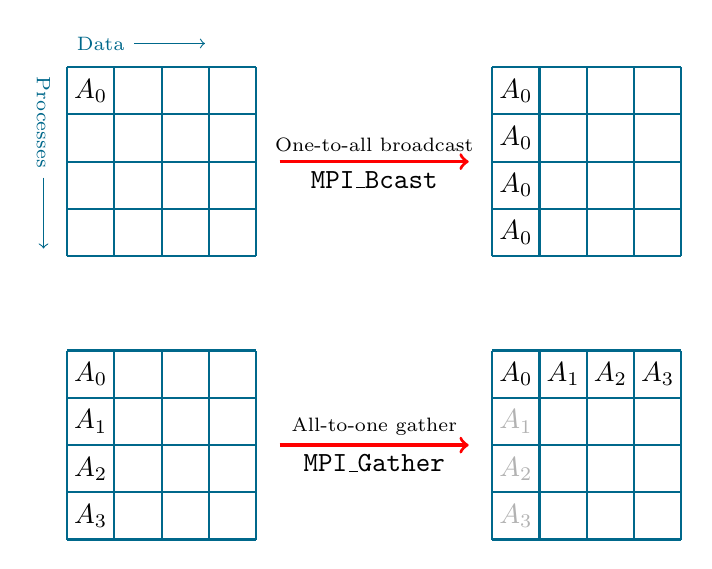
\begin{tikzpicture}[scale=0.6]
      \foreach \i in {0,...,4} {
        \foreach \j in {0,9} {
          \foreach \k in {0,6} {
            \draw[darkblue, thick] (\i+\j,0+\k) -- (\i+\j,4+\k);
            \draw[darkblue, thick] (0+\j,\i+\k) -- (4+\j,\i+\k);
          }
        }
      }
      \node at (0.5,9.5) {$A_0$};
      \node at (9.5,9.5) {$A_0$};
      \node at (9.5,8.5) {$A_0$};
      \node at (9.5,7.5) {$A_0$};
      \node at (9.5,6.5) {$A_0$};

      \node at (0.5,3.5) {$A_0$};
      \node at (0.5,2.5) {$A_1$};
      \node at (0.5,1.5) {$A_2$};
      \node at (0.5,0.5) {$A_3$};
      \node at (9.5,3.5) {$A_0$};
      \node at (10.5,3.5) {$A_1$};
      \node at (11.5,3.5) {$A_2$};
      \node at (12.5,3.5) {$A_3$};
      \node[color=black!30] at (9.5,2.5) {$A_1$};
      \node[color=black!30] at (9.5,1.5) {$A_2$};
      \node[color=black!30] at (9.5,0.5) {$A_3$};

      \draw[red, very thick, ->] (4.5,8) -- (8.5,8);
      \draw[red, very thick, ->] (4.5,2) -- (8.5,2);
      \node[anchor=north] at (6.5,8) {\texttt{MPI\_Bcast}};
      \node[anchor=south] at (6.5,8) {\scriptsize One-to-all broadcast};
      \node[anchor=north] at (6.5,2) {\texttt{MPI\_Gather}};
      \node[anchor=south] at (6.5,2) {\scriptsize All-to-one gather};

      \node[anchor=west, color=darkblue] (data) at (0,10.5) {\scriptsize Data};
      \node[anchor=west, color=darkblue, rotate=-90] (procs) at (-0.5,10) {\scriptsize Processes};
      \draw[darkblue, ->] (data.east) -- ($ (data.east) + (1.5,0) $);
      \draw[darkblue, ->] (procs.east) -- ($ (procs.east) - (0,1.5) $);
    \end{tikzpicture}
  \end{center}
\end{frame}

\begin{frame}
  \frametitle{Global reduction}
  \begin{center}
    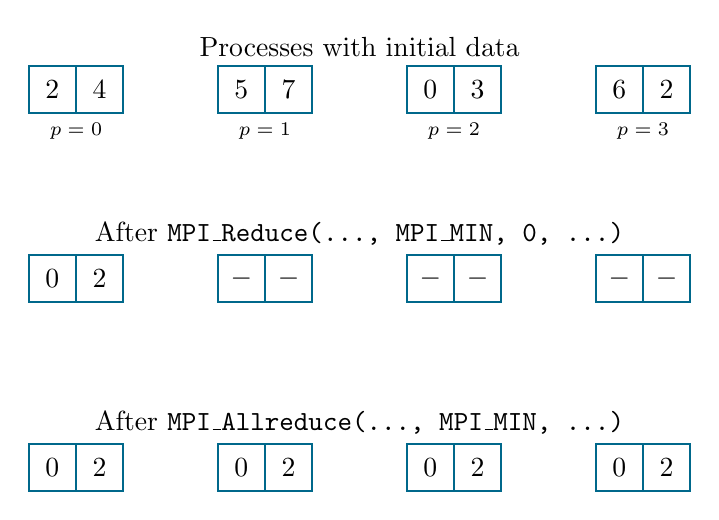
\begin{tikzpicture}[scale=0.6]
      \foreach \i in {0,4,8,12} {
        \foreach \j in {0,4,8} {
          \draw[darkblue, thick] (\i,\j) rectangle (\i+2,\j+1);
          \draw[darkblue, thin] (\i+1,\j) -- (\i+1,\j+1);
        }
      }

      \node[anchor=south] at (7,9) {Processes with initial data};
      \node[anchor=north] at (1,8) {\scriptsize $p=0$};
      \node[anchor=north] at (5,8) {\scriptsize $p=1$};
      \node[anchor=north] at (9,8) {\scriptsize $p=2$};
      \node[anchor=north] at (13,8) {\scriptsize $p=3$};
      \node at (0.5,8.5) {$2$}; \node at (1.5,8.5) {$4$};
      \node at (4.5,8.5) {$5$}; \node at (5.5,8.5) {$7$};
      \node at (8.5,8.5) {$0$}; \node at (9.5,8.5) {$3$};
      \node at (12.5,8.5) {$6$}; \node at (13.5,8.5) {$2$};

      \node[anchor=south] at (7,5) {After \texttt{MPI\_Reduce(..., MPI\_MIN, 0, ...)}};
      \node at (0.5,4.5) {$0$}; \node at (1.5,4.5) {$2$};
      \node at (4.5,4.5) {$-$}; \node at (5.5,4.5) {$-$};
      \node at (8.5,4.5) {$-$}; \node at (9.5,4.5) {$-$};
      \node at (12.5,4.5) {$-$}; \node at (13.5,4.5) {$-$};

      \node[anchor=south] at (7,1) {After \texttt{MPI\_Allreduce(..., MPI\_MIN, ...)}};
      \node at (0.5,0.5) {$0$}; \node at (1.5,0.5) {$2$};
      \node at (4.5,0.5) {$0$}; \node at (5.5,0.5) {$2$};
      \node at (8.5,0.5) {$0$}; \node at (9.5,0.5) {$2$};
      \node at (12.5,0.5) {$0$}; \node at (13.5,0.5) {$2$};
    \end{tikzpicture}
  \end{center}
\end{frame}

\begin{frame}
  \frametitle{Global reduction}
  \texttt{\textcolor{red}{MPI\_Reduce}($\underbrace{sbuf, rbuf, count, datatype}_{\textcolor{blue}{data}}$,
    $\underbrace{op, root, comm}_{\textcolor{blue}{envelope}}$); } \\
  \texttt{\textcolor{red}{MPI\_Allreduce}($\underbrace{sbuf, rbuf, count, datatype}_{\textcolor{blue}{data}}$,
    $\underbrace{op, comm}_{\textcolor{blue}{envelope}}$); }

  Examples of predefined operations (C):
  \begin{itemize}
  \item \texttt{MPI\_SUM}
  \item \texttt{MPI\_PROD}
  \item \texttt{MPI\_MIN}
  \item \texttt{MPI\_MAX}
  \end{itemize}
\end{frame}

\begin{frame}
  \frametitle{Overview}
  
\begin{itemize}
\item MPI provides a very expressive interface for Message Passing.
\item Basic routines are defined for data exchange and operations.
\item Extensions exist for parallel IO, shared memory, one-sided communication.
\item Each function may come in different flavours corresponding to various communication modes.
\item Ensuring proper scheduling of message to avoid deadlocks.
\item Packing the data for communication may require copy or creation of MPI Derived Types to define a ``view'' of the data.
\item Due to network latencies, communication patterns are crucial i.e profiling on a shared memory machine is not enough.
\end{itemize}

\end{frame}

\end{document}

